The purpose of this work is to study a short-time Fourier transform for its viability as a pitch detector. The FFT for transforming a waveform into the frequency-domain has been introduced and this chapter will focus on the properties of sound, introduce some musical terminology and how the FFT can be used to detecting pitches from a time-domain signal

\subsection{Basics of sound}
Sound physically is propagation through a medium, a vibration which some things can produce and some things can pick up. The word sound can be used to describe both the propagation itself, but also the phenomenom we feel when our ears react to the propagation. Speakers, strings of a guitar and vocal chords (together with the lungs) are some of the things that can produce sound and microphones and membranes in ears are things that can pick up sound. The propagation will have a certain strength at some point in the medium it travels through, which can be measured. This allows us to model the pressure propagation, or the sound as a function of time. At time $t$ the pressure at some point can be denoted as $f(t)$. This function over time can also be called a signal.

% source: https://api.pageplace.de/preview/DT0400.9781292055152_A24617782/preview-9781292055152_A24617782.pdf The Science of Sound - Rossing, Moore, Wheeler

One of the simplest ways to generate a sound is connecting a speaker to a device that generates an analog current in the shape of a wave. The current moves an electromagnet which moves a membrane at the same frequency as the generator. This membrane displaces air at some rate which ears pick up as sound. A 440Hz wave, a signal that oscillates 440 times per second that is, will produce a sound wave of 440Hz \todo{this most likely needs a source}. An ear picks up this signal as what we call an A4 note. Ironically, the purity of the signal makes it sound harsh and it is noise in the signal that gives warmth and beauty to the note. This can be observed in figure \ref{fig:pianoWave} where the signal (sound made by an electric piano) largely matches a pure A4 (440Hz sinusoid) but not quite.

%https://eprints.hud.ac.uk/id/eprint/17816/1/Final_Thesis_-_November_2012.pdf

\begin{figure}[ht]
    \centering
    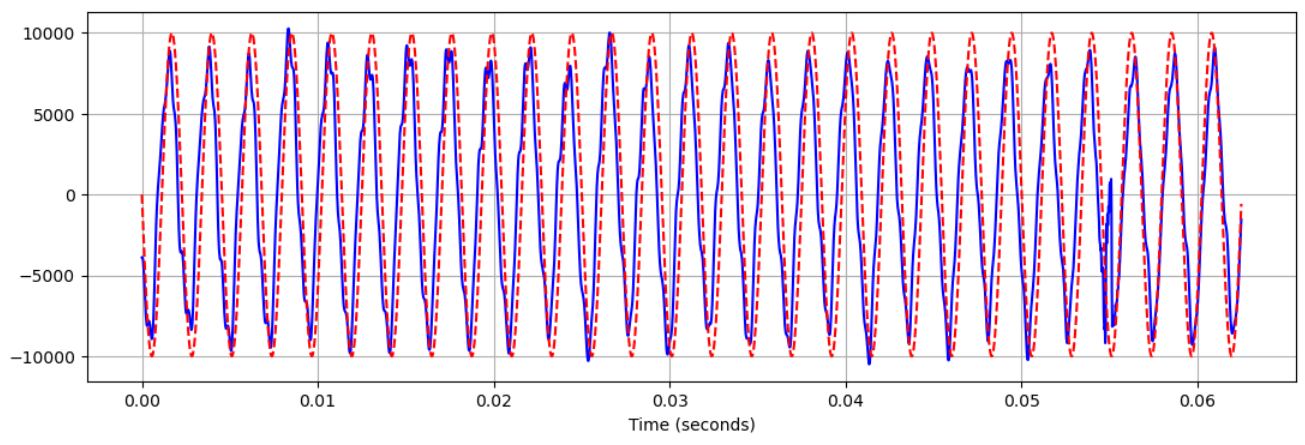
\includegraphics[width=\textwidth]{./images/piano_wave.png}
    \caption{A slice of the recording of a A4 note played on a Yamaha electric piano (blue solid). The signal contains a lot of irregularity but also clear regularity which becomes more evident when layering a pure A4 note on top (red dashed).\label{fig:pianoWave}}
\end{figure}

The characteristics of the sound being played becomes even more evident when it's converted to the frequency-domain through the FFT as shown in figure \ref{fig:pianoFreq}. It reveals that, not only is the sound definitely a A4 note due to the overwhelming amount of the 440Hz signal present in the sound, but also what other frequencies contribute to the sound of that piano. The spectrum also reveals that the particular electric piano that was used to create the sound lacks harmonic content.

\begin{figure}[ht]
    \centering
    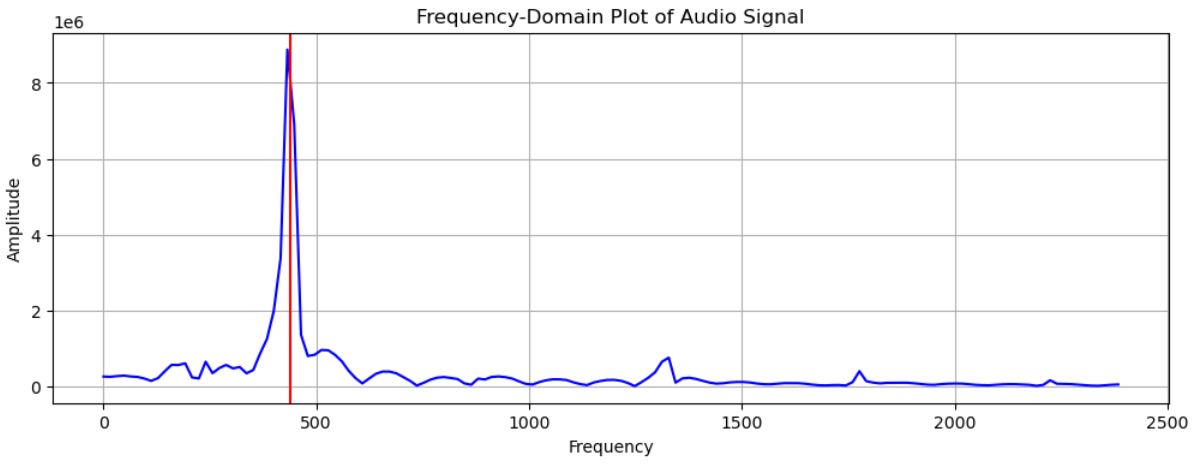
\includegraphics[width=\textwidth]{./images/piano_freq.png}
    \caption{The frequency-domain clearly reveals without any guesswork that the signal is a 440Hz signal with some sort of noise/disturbance. The red vertical line is placed at $x=440$ to show that the peak is the expected 440Hz frequency component.\label{fig:pianoFreq}}
\end{figure}

\subsubsection{Semitones, notes and pitch} 
Music terminology can be hard to define without circular definitions. There's also quite a bit of overlap with the same word meaning different things depending on context. We can start with defining the octave which is the difference between two sounds where one sound has twice the frequency of the other and is the largest interval in western music. If a sound oscillates at 440Hz, the sounds corresponding to 220Hz or 880Hz are an octave away.

Semitone is typically defined as the smallest interval in western music and is 1/12th of an octave. Semitone is sometimes also used to talk about, not the interval, but the sounds that bound the interval. This non-interval semitone is sometimes also called a pitch and sometimes note.

In western music, tuning typically starts from A4, which is defined in this system to have a frequency of 440Hz, and every other note is derived from there. A3 (an octave lower) will be 220Hz and A5 will be 880Hz. The frequency for the other pitches can be approximated with equal temperament tuning, meaning that all semitones are equally spaced within octaves. This means that the frequency of any one pitch is exactly $2^{1/12}$ times the frequency of the previous one. Sounds are given identifiers as a letter-number pair based on the octave they are in and their placement within the octave. 

\subsubsection{Terminology for readers}
In this work, the term "note" will be used to describe the base notes and the base notes will be defined according to German/European music theory as \[C, D, E, F, G, A, H\] and B being $H\flat$. The term "semitone" will be used to describe all the 12 distinct sounds in an octave, including the sharps/flats of the notes. In other words, the notes are a subset of the semitones. Pitch will be used to describe the measurement/perception of how low or high a sound is. 

% \subsubsection{Pitch perception}
% Even though we can clearly define any one pitch to be some frequency, human ears are more complex. 
% What do I want to establish in this chapter????
% What is pitch perception at a high level
% 
\subsection{Fundamental frequency estimation}
Even though we can define a pitch to be a precise frequency, pitch is more of a sensation perceived by ears and we can distinguish pitch from soundwaves that are not simple oscillations. As shown in \ref{fig:pianoWave}, what we perceive as an A440 can contain a lot of noise.  As it can be difficult to strictly define pitch, pitch detection may also be hard to define. From a computational perspective, a possible definition is that pitch detection is the identification of the fundamental frequency and which is the corresponding semitone (because the sound names are more valuable to musicians than the pure frequencies). The fundamental frequency is typically the lowest frequency of a signal, but in some cases we can hear a fundamental frequency that isn't actually a part of the signal, a phenomenon appropriately called the missing fundamental. \todo{source: Gotsopoulos}. An example of this would be telephones, that could not record below 300Hz. Male voices would still sound male, even though their fundemental frequency of around 150Hz was completely missing \todo{Mather 2006}. 

\subsection{Pitch detection methods}
Pitch detection methods typically fall into one of 3 categories: time-domain, frequency-domain and statistical/ML methods.

\subsection {Transforming to frequency-domain}
\subsubsection{Short-time Fourier Transform}
The short-time Fourier Transform (STFT) is a method of analysing local frequency data by transforming only a portion of a given signal. The STFT is typically defined very similarly to the FT/DFT only with a windowing function applied. The discrete STFT conceptually computes the DFT for a window of the signal, then moves the window over some number of steps (called the hop length) and repeats. The next window may or may not overlap with the previous window.

This sliding window introduces a new dimension to the output data, a time axis. This data constitutes a spectrogram and the typical way to visualize this data is with a heat map by compressing the 2D of the frequency-domain to a column where intensity represents the magnitude value for a frequency. 

\begin{figure}[ht]
    \centering
    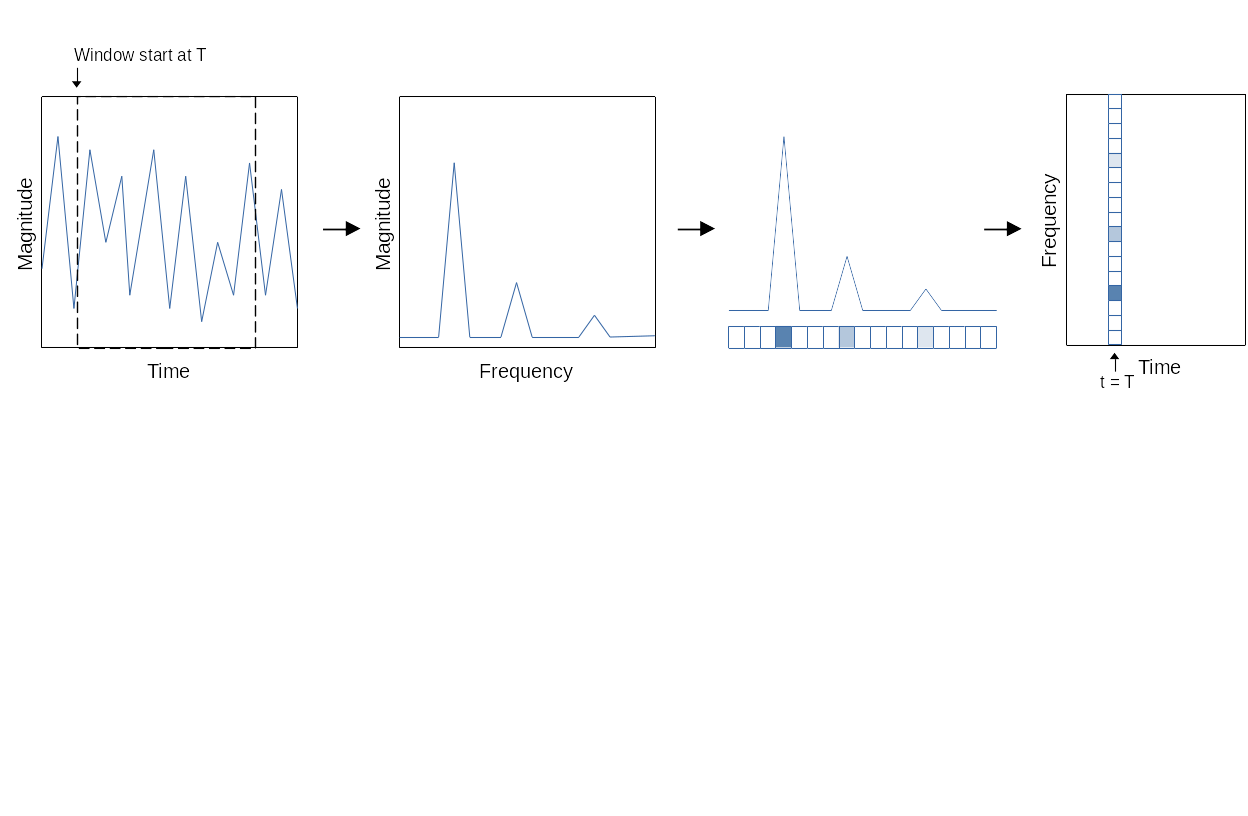
\includegraphics[width=\textwidth]{./images/stft.png}
    \caption{High level overview of the SFTF. The STFT performs the DFT for every window which results in a spectrogram. For ease of visualization, the frequency-domain is typically visualized using color intensity for the magnitude. \label{fig:stft}}
\end{figure}

It's worth pointing out that the STFT is not a special kind of fourier transform, but rather a method of applying the DFT (or contiunuous FT). This means it has the same behaviour but also that it has the problems which will be introduced shortly. 

For real-time processing, it's both imperetive and a bit redundant to talk about the STFT because the entirety of the signal is not availabl, there will inherently be windows. The data will be available as a stream (or chunks) and an FFT can be performed once a buffer is filled. The overlap, which is determined by the hop length, doesn't seem to be of much importance for the purpose of the estimating the fundamental frequency and makes little sense when the data becomes available with time. The overlap is important when considering note lengths and separation of repeated semitones \todo{Evans, Benjamin Peter, PhD}, but does not seem to be a concern for just pitch detection. The pitch detector will thus have a hop length the size of the window.

\subsection{Picking peaks from the spectrum}
The Fourier transform is used to get the spectrum data, which can be used to plot which frequencies are part of the original signal. These frequencies that are part of the signal are called partials. Intuitively, for a lot of signals, anyone can look at the frequency-magnitude plot and point to a peak and claim that it's the fundamental frequency and probably be right. Perhaps they are looking for some periodicity with the largest peaks (if there are multiple) and choosing out of those the peak that has the lowest frequency. This is a very straightforward approach and correct for some signals. 
\subsubsection{Harmonic Product Spectrum}
Harmonic Product Spectrum (HPS) is an algorithm that does almost does the intuitive approach. 
$$Y = \prod_{r=2}^R X_r$$ where $X_r$ denotes the signal X downsampled by r. Simply put, the HPS iteratively multiplies downsampled version of a signal. Downsampling the frequency-domain effectively compresses the frequency-axis by the downsampling rate which means that previously integer multiplies of some value $kN$ are put in the same bins as $N$. When all the downsampled frequency-domain signals are multiplied together, correlated frequencies, or harmonics, form a very sharp peak \cite{McLeod2008}. This peak can be picked out with a max function.

\begin{figure}[ht]
    \centering
    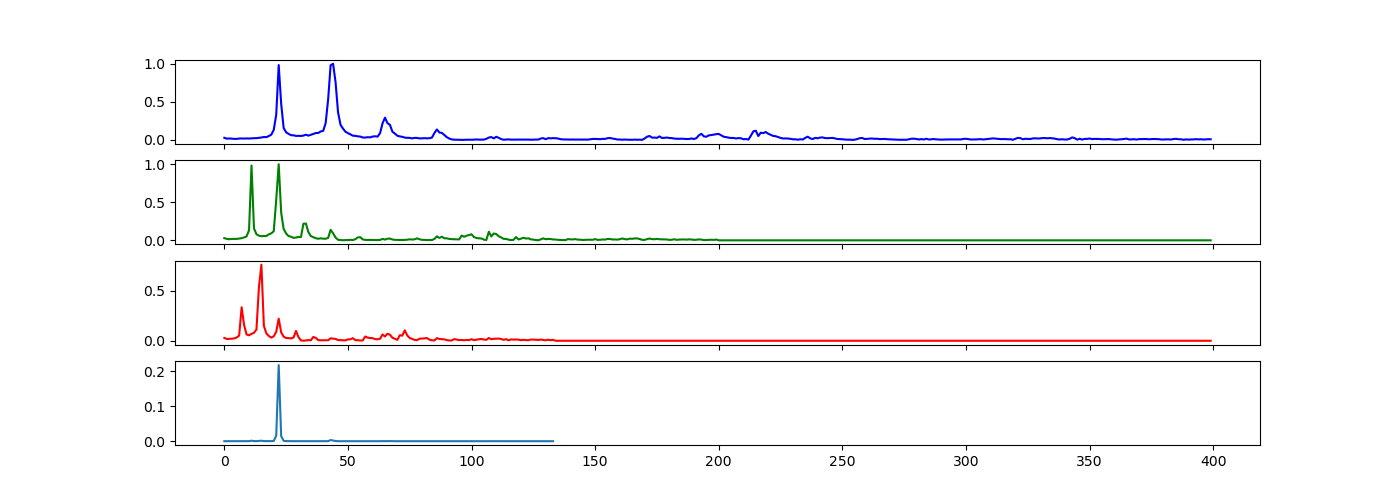
\includegraphics[width=\textwidth]{./images/hps.png}
    \caption{Plot of signal and downsampled versions of it and the final HPS. Harmonics align and form a peak. \label{fig:hps}}
\end{figure}

HPS is a good algorithm because it's simple and easy to compute making it suitable for real-time analysis. It also has the ability to 
One problem with the HPS is that it does not perform well in the case of lacking harmonics \cite{McLeod2008}. This likely won't be a problem because human voices should be rich in harmonic content. According to \cite{Smyth2019}, the HPS is also prone to getting octaves wrong, but that did not seem to be the case when testing preliminarily with guitar, piano and a voice.

% Problems with FFT, might move this to real-time
\subsection{Problems with the FFT}
\subsubsection{Frequency bin sizes}
One problem with the FFT that  \todo{source: Gotsopoulos} addresses is the size of the frequency bins. This is also noted for the STFT, limiting how short the STFT can be for achieving sufficient frequency resolution \todo{Evans, Benjamin Peter, PhD}. The FFT doesn't find precise frequencies, it finds bins of frequencies with the size $S/N$ where S is the sampling rate and N is the FFT buffer size. As frequency grows exponentially (doubles every octave), higher notes are spaced further apart. This means that for lower notes, the frequency bins need to be significantly smaller as shown in figure \ref{fig:fftBinSizeChart}. Base singers may need to go very low, around F2 (87Hz) and in order to avoid notes in this range to fall into the same bin, the window size needs to be very small.  

\begin{figure}[ht]
    \centering
    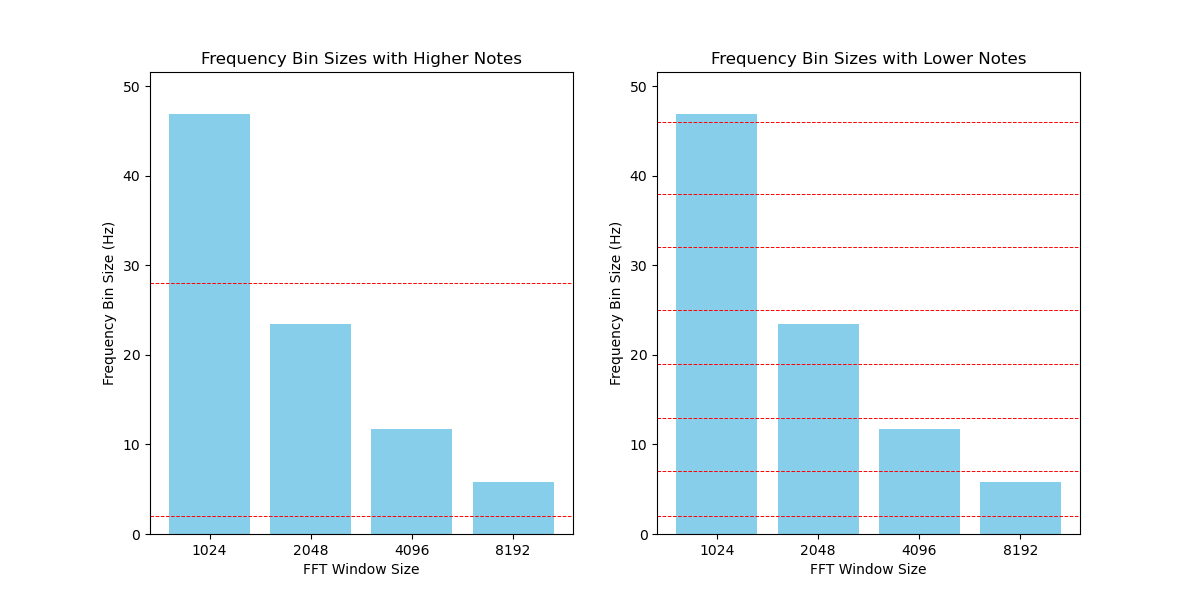
\includegraphics[width=\textwidth]{./images/fft_bin_size_chart.png}
    \caption{As the FFT window shrinks, different notes may fall into the same bin. Bars represent the bin sizes for various window sizes at 48kHz sampling rate and dashed lines show semitone intervals (the exact note values are irrelevant). For notes in the 4th octave, the window size can be smaller, but in the 2nd octave even 8192 samples is not enough to discern all pairs of semitones because the bins are larger than those semitone differences.\label{fig:fftBinSizeChart}}
\end{figure}

Base singers typically go as low as E2 and the difference between E2 and F2 is barely 5Hz which is smaller than the frequency bin of 8192 samples at 48kHz. They do not necessarily fall into the same bin but it would be safer to compute the FFT with a 16384 window size. This halves the frequency bin size and definitely accomodates differences even an octave lower. This introduces a significant amount of increased computation and is quite unnecessary as base singers do not realistically go this low. If the FFT implementation allows (many implementations require a power of 2), the window size should lie somewhere between 8192 and 16384 to lessen computations. For a 4Hz bin, $48000/x = 4 <=> x = 48000/4 = 12000$ 12000 samples would be enough to discern the lowest notes. 

This introduces another problem, which has implications for real-time pitch detection which is that collecting 12000 samples at 48kHz takes 0.25s, which arguably is not real-time anymore. As the bin size is $B = S/W$ means that $W = S/B$ and the latency (time taken to fill the FFT window) $L = W/S = \frac{S/B}{S} = 1/B$, the bin size and latency are inversely proportional, both can not be minimized. For a bin size of 4, it will necessarily take 0.25s to collect the FFT samples. This follows that naively transforming audio makes real-time pitch detection for base singers impossible, the detection latency will inherently always be too long.

% Narrowing the problem
\subsection{Real-time pitch detection}
One challenge with real-time pitch detection that emerged from the problem with the size of frequency bins was that for detecting lower base notes, the window size needed to be around 12000. However collecting 12000 samples at 48kHz takes 0.25s, which arguably is not real-time anymore. It takes 0.33s if for any reason the window size needs to be 16384. If the window size is made smaller, the resulting FFT will have larger bins than what is necessary for detecting lower frequencies. 
\subsubsection{Zero-padding}
A popular approach to increasing frequency resolutions is to pad the end of the signal with zeros. Zero-padding makes the signal longer and while it necessararily introduces frequency components, the peaks remain intact. This allows a larger FFT window that, while increasing computational complexity, allows for better frequency resolution as per the previous equations. At 48kHz, 16000 samples are enough to achieve a 3Hz frequency bin. If out of these 16000, 10000 are zeros and 6000 legitimate datapoints, the FFT window can be "filled" in a mere 125ms which is a more acceptable latency for real-time detection. Figure \ref{fig:zeropadSpectrum} shows how zero-padding affects the spectrum.

\begin{figure}[ht]
    \centering
    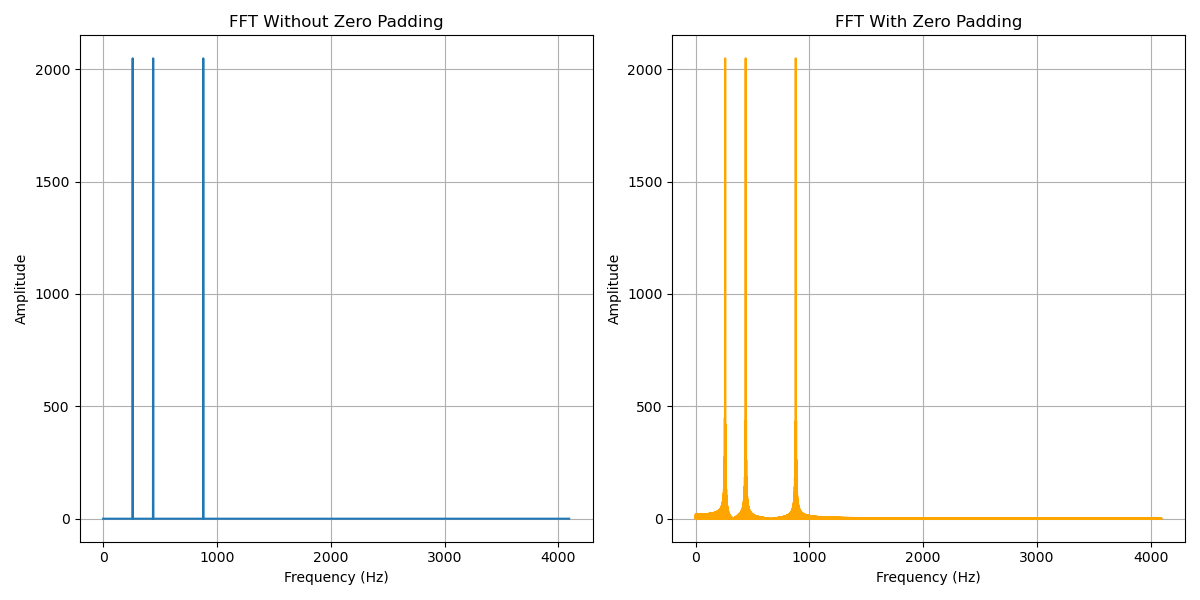
\includegraphics[width=\textwidth]{./images/zero_pad_spectrum.png}
    \caption{Spectrum contents of a signal consisting of 260, 440 and 880 frequency components. While the zero-padding introduces a small amount of frequency data around the peaks, the peaks themselves are not affected. \label{fig:zeropadSpectrum}}
\end{figure}

\subsubsection{Reducing sampling rate and window size}
As the bin size is the ratio of the sampling rate to number of samples, $B = S/N$, reducing both $N$ and $S$ keeps the bin size small. 
\subsection{Finding nearest semitone}
%https://newt.phys.unsw.edu.au/jw/notes.html
As already established, western tuning is done in equal temperaments, meaning the octave is evenly divided in 12. Using A4 (440Hz) as a reference, one can calculate every semitone's frequency with a signed index from A4 using the following function. 
$$f(i) = 2^{i/12}*440$$
For example the -2-th semitone using the formula is approximately G4 which indeed is 2 semitones under A4. To avoid negative indices, they can be shifted by some number. A4 is assigned the MIDI (Musical Instrument Digital Interface) number 69 so this will be the number the scale gets shifted by. So to find the frequency of the i-th semitone the following function can be used.
$$f(i) = 2^{\frac{i-69}{12}}*440$$
To find the frequency for a MIDI number, the function can be rewritten as a function of $f$.
First divide both sides by 440
$$f/440 = 2^{\frac{i-69}{12}}$$
then remove the exponent using a logarithm
$$\log_2(f/440) = \log_2(2^{\frac{i-69}{12}}) = \frac{i-69}{12}$$
then divide both sides by 12
$$12*\log_2(f/440) = i-69$$
and finally subtracting 69 from both sides and giving an appropriate identifier for the function, like M for MIDI number, the final formula for calculating the MIDI number for a frequency is.
$$M(f) = 12*\log_2(f/440)+69$$
While the MIDI numbers are discrete, the derived formula interpolates between the MIDI numbers. If the input is a number that isn't a semitone, like 450, the result is $M(450) \approx 69.4$. This can be rounded to the nearest integer.

The function that will be used in the pitch detector is
$$M(f) = round(12*\log_2(f/440)+69)$$

